\documentclass[11pt,a4paper]{article}
\usepackage[margin=2.35cm]{geometry}
\usepackage{amsmath,booktabs,graphicx,array,float,hyperref}
\usepackage[table]{xcolor}
\hypersetup{colorlinks=true,linkcolor=blue,urlcolor=blue}
\setlength{\parskip}{0.35em}
\newcommand{\param}[1]{\texttt{\detokenize{#1}}}
\title{Assignment 2\\Parameter Perturbation Plan and Experiment Record}
\author{Mathematical Methods in Uncertainty Quantification}
\date{Living document}
\begin{document}
\maketitle
\section{Model and baseline}
We use the HBV001a model, calibration bounds, and saved optimal parameters from the specified Assignment 1 folder. Evaluation retains the Assignment 1 settings: \(J=1-\mathrm{NSE}\), with no warm-up. The reproduced baseline is
\[J^*=0.0927763,\qquad \mathrm{NSE}^*=0.907224.\]
The original calibration bounds are hard limits. All perturbations start from this parameter vector. If a different random seed supplies a different vector, feasible ranges must be checked again.
\section{Parameter perturbation classification and treatment}
All 18 calibrated quantities are varied one at a time. A small numerical value does not imply low sensitivity: \param{lrr_dre} is approximately 0.00913 and ranks third. Parameters have different units and meanings, so numerical magnitude alone is not grounds for exclusion.
\subsection{Parameters that permit both 20\% endpoints}
The following 12 parameters remain within their calibration bounds when multiplied by 0.8 or 1.2: \param{snw_att}, \param{snw_pmf}, \param{snw_amf}, \param{sl0_bt0}, \param{urr_dth}, \param{lrr_dth}, \param{urr_ulc}, \param{urr_tdh}, \param{urr_tdr}, \param{urr_ndr}, \param{urr_uct}, and \param{lrr_lct}.
\subsection{Parameters constrained by calibration bounds}
Each side changes by at most 20\%. If a bound is reached first, the perturbation stops there. Actual endpoint changes are shown below.
\begin{center}\small
\begin{tabular}{lrrrr}\toprule
Parameter & Baseline & Calibration range & Lower direction & Upper direction\\\midrule
\param{snw_dth} & 8.58808 & 0--10 & $-20\%$ & $+16.44\%$\\
\param{sl0_dth} & 49.06446 & 0--50 & $-20\%$ & $+1.91\%$\\
\param{sl0_pwp} & 646.54862 & 5--700 & $-20\%$ & $+8.27\%$\\
\param{sl0_fcy} & 122.27323 & 100--700 & $-18.22\%$ & $+20\%$\\
\param{urr_wsr} & 0.99104 & 0--1 & $-20\%$ & $+0.90\%$\\
\param{lrr_dre} & 0.00913049 & 0--0.01 & $-20\%$ & $+9.52\%$\\\bottomrule
\end{tabular}
\end{center}
Feasible ranges differ; the positive ranges for \param{sl0_dth} and \param{urr_wsr} are especially narrow.
\subsection{Temperature threshold}
The baseline \param{snw_att} is approximately $-0.00604556\,^\circ\mathrm C$. Multiplication by 0.8 and 1.2 yields approximately $-0.00483645$ and $-0.00725467\,^\circ\mathrm C$, each about $0.00120911\,^\circ\mathrm C$ from baseline. Since the baseline is negative, multiplying by 1.2 lowers the temperature. Percentage changes also require caution because the Celsius scale has an arbitrary zero. Larger absolute temperature changes have not been tested.
\section{One-at-a-time local sensitivity}
One parameter is changed at a time with all others fixed. Each side has 10 equally spaced points plus the baseline: 21 per parameter, or 378 records. The relative objective change and ranking score are
\[\Delta J(\%)=100\frac{J(\theta_i')-J^*}{J^*},\qquad S_i=\frac{1}{20}\sum_{k=1}^{20}|\Delta J_{i,k}(\%)|.\]
\(S_i\) is the mean absolute objective change over the 20 non-baseline points. Feasible ranges differ, so rankings are not comparisons under identical perturbation ranges.
\begin{center}\small
\begin{tabular}{rlrr}\toprule
Rank & Parameter & Mean absolute change & Relative perturbation range\\\midrule
1 & \param{sl0_fcy} & 5.8126\% & $-18.22\%$ to $+20.00\%$\\
2 & \param{snw_pmf} & 4.7719\% & $-20.00\%$ to $+20.00\%$\\
3 & \param{lrr_dre} & 4.2247\% & $-20.00\%$ to $+9.52\%$\\
4 & \param{sl0_bt0} & 0.70836\% & $-20.00\%$ to $+20.00\%$\\
5 & \param{sl0_dth} & 0.6923\% & $-20.00\%$ to $+1.91\%$\\
6 & \param{snw_amf} & 0.49607\% & $-20.00\%$ to $+20.00\%$\\
7 & \param{snw_att} & 0.36891\% & $-20.00\%$ to $+20.00\%$\\
8 & \param{urr_ulc} & 0.33188\% & $-20.00\%$ to $+20.00\%$\\
9 & \param{urr_wsr} & 0.10211\% & $-20.00\%$ to $+0.90\%$\\
10 & \param{snw_dth} & 0.040245\% & $-20.00\%$ to $+16.44\%$\\
11 & \param{sl0_pwp} & 0.0048632\% & $-20.00\%$ to $+8.27\%$\\
12 & \param{lrr_dth} & 0.0034587\% & $-20.00\%$ to $+20.00\%$\\
13 & \param{lrr_lct} & 0.0026344\% & $-20.00\%$ to $+20.00\%$\\
14 & \param{urr_uct} & 0.0014379\% & $-20.00\%$ to $+20.00\%$\\
15 & \param{urr_dth} & 0.00095492\% & $-20.00\%$ to $+20.00\%$\\
16 & \param{urr_ndr} & 0.00075207\% & $-20.00\%$ to $+20.00\%$\\
17 (tie) & \param{urr_tdh} & 0\% & $-20.00\%$ to $+20.00\%$\\
17 (tie) & \param{urr_tdr} & 0\% & $-20.00\%$ to $+20.00\%$\\
\bottomrule
\end{tabular}
\end{center}
For \param{snw_att}, the mean absolute change is about 0.369\%, showing a measurable response in this experiment. This concerns only the tiny relative perturbation above and cannot predict the impact of larger absolute temperature changes. \param{urr_tdh} and \param{urr_tdr} produced no objective change at the tested points; this need not hold under other conditions.
\section{How the three highest-ranked parameters affect the model}
The objective sums squared errors between simulated and observed discharge over time. Perturbations can change both the magnitude and timing of these errors. Both tested endpoints of the three highest-ranked parameters increased \(J\).
\subsection{\param{sl0_fcy}: soil field capacity}
This parameter affects soil storage capacity and the fraction of incoming water producing runoff. It can change the amount and timing of water entering reservoirs, thereby affecting simulated discharge and the objective.
\subsection{\param{snw_pmf}: precipitation-induced melt factor}
With snow present, precipitation, and temperature above the threshold, this factor controls precipitation-induced melt. Perturbation may alter the timing and amount of meltwater reaching the soil and the resulting discharge. Total melt is also limited by remaining snow and the air-induced melt process.
\subsection{\param{lrr_dre}: lower-reservoir channel outflow coefficient}
This coefficient affects the release rate from the lower reservoir. An increase generally releases more of the current storage, leaving less for later time steps and potentially changing the hydrograph.
These pathways follow the model equations. The timing and flow features responsible for the objective changes require inspection of hydrographs.
\section{Preliminary explanation of low sensitivity}
\param{urr_tdh} and \param{urr_tdr} control the upper reservoir fast-outlet threshold and coefficient. In the baseline, maximum storage immediately before the fast-outlet calculation was approximately 18.12 mm, below the lowest tested threshold of 78.79 mm. The fast outlet was not activated, so changing these parameters within the tested range had no effect on the objective.
The normal upper outlet controlled by \param{urr_ndr} conveyed about 0.009 mm during the baseline period. Upper and lower subsurface exports totalled about 0.034 and 0.065 mm and are not added directly to calibrated channel discharge; \param{urr_uct} and \param{lrr_lct} therefore also have small effects here. \param{urr_dth} and \param{lrr_dth} set initial storage; their effects may weaken over time, which requires hydrograph verification. \param{sl0_pwp} controls soil moisture limitation of evapotranspiration. Actual evapotranspiration was about 3.35 mm, versus precipitation of about 299.20 mm; this is a plausible explanation for its small effect in this period.
\section{Combined perturbations of the three highest-ranked parameters}
We evaluated 12 two-parameter endpoint combinations and eight three-parameter combinations for \param{sl0_fcy}, \param{snw_pmf}, and \param{lrr_dre}. The baseline, model, and endpoints are unchanged, and the results have been recalculated.
Their lower and upper endpoints are, respectively: \param{sl0_fcy} $-18.22\%$, $+20\%$; \param{snw_pmf} $-20\%$, $+20\%$; and \param{lrr_dre} $-20\%$, $+9.52\%$. The following table shows relative \(J\) changes; signs follow parameter order.
\begin{center}\small
\begin{tabular}{lrrrr}\toprule
Parameter pair & $-/-$ & $-/+$ & $+/-$ & $+/+$\\\midrule
\param{sl0_fcy} / \param{snw_pmf} & 26.75\% & 25.24\% & 31.20\% & 25.78\%\\
\param{sl0_fcy} / \param{lrr_dre} & 20.09\% & 23.05\% & 49.52\% & 12.48\%\\
\param{snw_pmf} / \param{lrr_dre} & 34.86\% & 16.29\% & 29.52\% & 12.83\%\\\bottomrule
\end{tabular}
\end{center}
For three parameters, the order is \param{sl0_fcy} / \param{snw_pmf} / \param{lrr_dre}:
\begin{center}\small
\begin{tabular}{lrlr}\toprule
Direction & Change in \(J\) & Direction & Change in \(J\)\\\midrule
$-/-/-$ & 34.06\% & $+/-/-$ & 64.92\%\\
$-/-/+$ & 34.62\% & $+/-/+$ & 26.13\%\\
$-/+/-$ & 32.13\% & $+/+/-$ & 58.82\%\\
$-/+/+$ & 34.67\% & $+/+/+$ & 22.08\%\\\bottomrule
\end{tabular}
\end{center}
With \param{sl0_fcy} and \param{lrr_dre} both at their upper endpoints, individual effects are 16.47\% and 2.92\%, summing to 19.38\%; their combined change is 12.48\%, indicating partial cancellation. With all three at their upper endpoints, individual changes sum to 29.13\% while the combined change is 22.08\%. Three-parameter departures include pairwise and higher-order effects. None of the 20 endpoint combinations returns exactly to baseline; stronger cancellation at intermediate values remains possible.
\clearpage
\section{Perturbation curves and sensitivity ranking}
Each point varies one parameter while others remain at baseline. The horizontal axis is relative parameter change and the vertical axis is relative objective change. Since the temperature threshold is negative, positive percentage change means a more negative temperature. Feasible horizontal ranges are not necessarily symmetric.
\begin{figure}[H]\centering\includegraphics[width=\textwidth]{figures/perturbation_curves_1.png}\caption{One-at-a-time perturbation curves for the first nine parameters.}\end{figure}
\begin{figure}[H]\centering\includegraphics[width=\textwidth]{figures/perturbation_curves_2.png}\caption{One-at-a-time perturbation curves for the remaining nine parameters.}\end{figure}
\begin{figure}[H]\centering\includegraphics[width=0.93\textwidth]{figures/sensitivity_ranking.png}\caption{Ranking by mean absolute objective change over each parameter's feasible range.}\end{figure}
\clearpage
\section{Hydrograph comparison for the three highest-ranked parameters}
Each figure compares observed discharge, the baseline, and simulations at both perturbation endpoints, holding all other parameters fixed. The upper panel shows the full time series. The lower panel shows a 72-hour diagnostic window selected by maximizing the sum, across both endpoints and the window, of the absolute hourly changes in squared error. This highlights visible changes but does not necessarily maximize the net objective contribution.
The legend reports actual parameter changes and the corresponding full-period objective changes. Hourly squared-error changes can be positive or negative, and periods can offset one another. Hydrograph separation alone does not establish the net objective effect.
\begin{figure}[H]\centering\includegraphics[width=\textwidth]{figures/hydrograph_sl0_fcy.png}\caption{Discharge response to soil field capacity.}\end{figure}
The \param{sl0_fcy} diagnostic window is 12--15 January 2011. The upper endpoint's net squared-error increase in this window is about 20.9\% of its full-period net increase. The lower endpoint instead reduces net error in the window, although its full-period objective increases. Different periods can therefore have opposite effects.
\begin{figure}[H]\centering\includegraphics[width=\textwidth]{figures/hydrograph_snw_pmf.png}\caption{Discharge response to the precipitation-induced melt factor.}\end{figure}
The \param{snw_pmf} diagnostic window is 11--14 January 2011. The lower endpoint's net squared-error increase in this window is about 74.1\% of its full-period net increase. The upper endpoint reduces net error in this window, although its full-period objective still increases.
\begin{figure}[H]\centering\includegraphics[width=\textwidth]{figures/hydrograph_lrr_dre.png}\caption{Discharge response to the lower-reservoir channel outflow coefficient.}\end{figure}
The \param{lrr_dre} diagnostic window is 7--10 January 2011. The lower endpoint's net squared-error increase in this window is about 82.5\% of its full-period net increase. The upper endpoint reduces net error in the window, while its full-period objective increases. These ratios use signed error changes, so positive and negative periods can offset; they are not fractions of all absolute error changes.
The figures confirm that these parameters can alter hydrographs and identify periods with substantial changes. The causal pathways through soil storage, melt, and reservoir release come from the model equations; internal states must be examined to verify each individual event.
\clearpage
\section{Differential evolution calibration with time-weighted objective}
Use fixed weights obtained by minimizing the worst relative response over 60 perturbation points around the original vector, with minimum weight 0.7 for the highest 10\% of observed flows and 0.1 otherwise. Differential evolution recalibrates within the original bounds with the original vector included as an initial candidate and the same random seed. The original early-convergence criterion was disabled and the run reached 700 generations, with 100944 objective evaluations.
\begin{center}\begin{tabular}{lrr}\toprule
Metric & Original & Weighted DE, 700 generations\\\midrule
Weighted objective & 0.102420 & 0.099737\\
Standard NSE & 0.907224 & 0.902678\\
Simulation at maximum observed peak ($\mathrm{m^3/s}$) & 105.39 & 105.26\\\bottomrule\end{tabular}\end{center}
The observed value at that time is 153.50 $\mathrm{m^3/s}$. The run stopped at its generation limit, not by the usual convergence criterion, and does not establish a global optimum. Standard NSE and peak comparisons are for the calibration period; no independent validation was performed.
\begin{figure}[H]\centering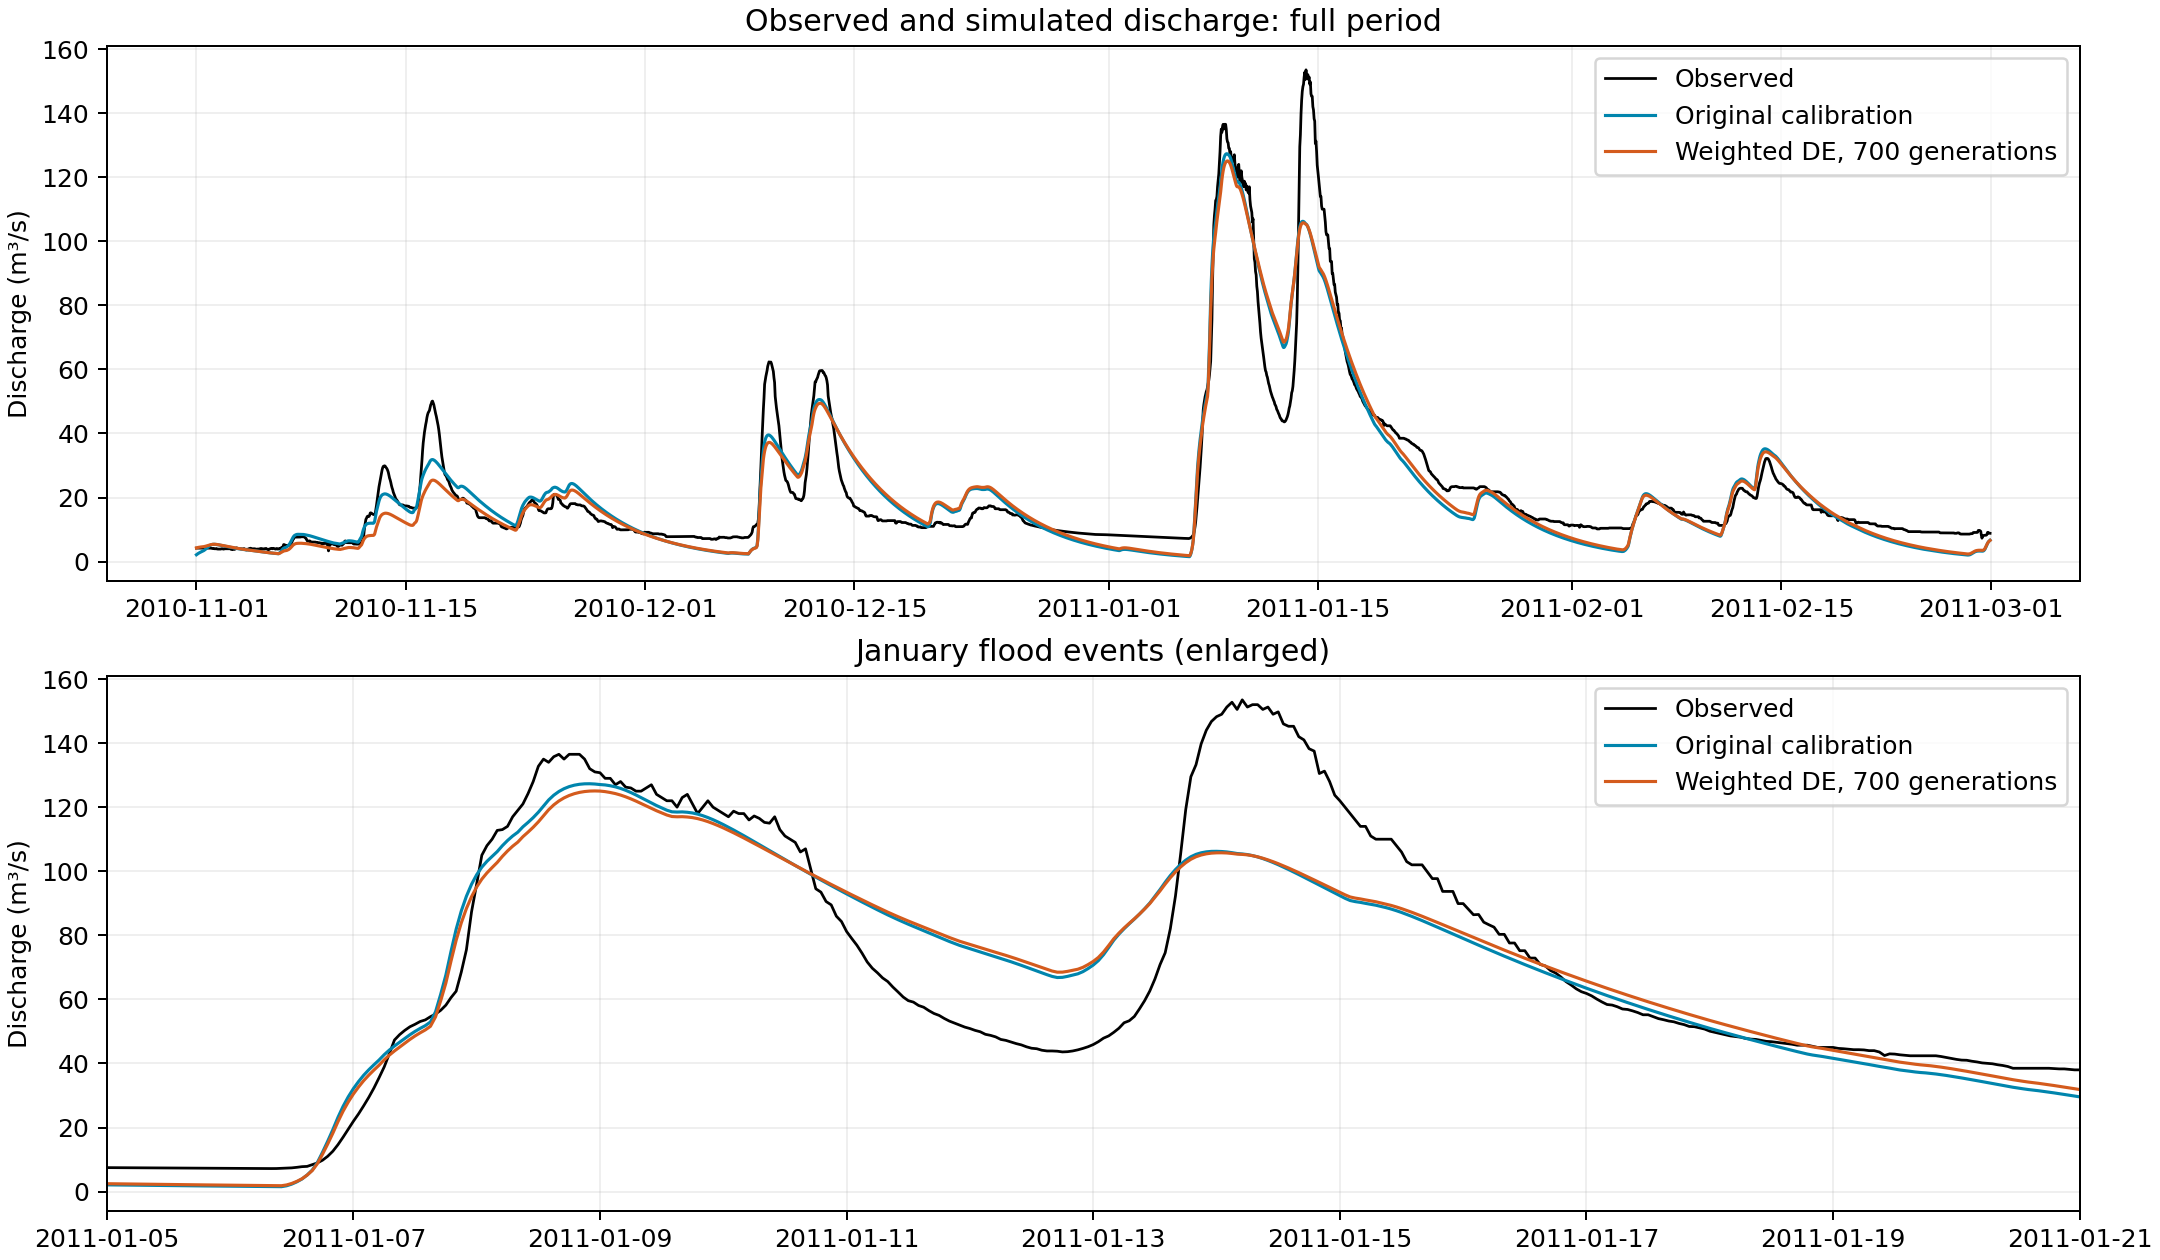
\includegraphics[width=\textwidth]{figures/weighted_de_700_fit.png}\caption{Original calibration and the time-weighted differential-evolution fit.}\end{figure}
\clearpage
\subsection{Sensitivity before and after the adjustment}
The original columns use the original vector and $J=1-\mathrm{NSE}$; the weighted columns use the new vector and the fixed-weight objective. Each column uses 20 non-baseline perturbations around its respective vector. The mean is the mean absolute relative objective change; the maximum is the largest absolute relative change.
\begin{center}\small\begin{tabular}{lrrrr}\toprule
Parameter & Original mean & Original max & Weighted mean & Weighted max\\\midrule
\param{sl0_fcy} & 5.81\% & 16.47\% & 4.63\% & 12.89\%\\
\param{snw_pmf} & 4.77\% & 14.64\% & 4.02\% & 11.96\%\\
\param{lrr_dre} & 4.22\% & 19.42\% & 4.76\% & 16.84\%\\\bottomrule\end{tabular}\end{center}
All three maxima decrease, but none is below 10\%; the mean for \param{lrr_dre} increases. The approximately 10\% limit around the original vector did not hold after recalibration. Weights were designed from original perturbation points and about 31.5\% of hours are near the minimum; high-flow protection does not guarantee improved peak fitting. Objectives and baselines differ, and feasible perturbation ranges may differ, so these relative changes are not changes in standard NSE.


\clearpage
\section{Recalibration with absolute-error objective}
Both numerator and denominator use absolute deviations, with the observed mean as the denominator reference:
\[J_{\mathrm{abs}}=\frac{\sum_t|Q_t^{\mathrm{sim}}-Q_t^{\mathrm{obs}}|}{\sum_t|Q_t^{\mathrm{obs}}-\overline Q^{\mathrm{obs}}|}.\]
This is absolute error at every time step, distinct from Huber loss, which is quadratic for small residuals and linear for large residuals. Differential evolution starts from a Latin-hypercube random population without inserting the original best vector. The original calibration bounds, population multiplier 8, and random seed 42 are retained. Early stopping was disabled and the run reached 700 generations and 100944 evaluations. It stopped at the generation limit, without establishing natural convergence or a global optimum.
\begin{center}\begin{tabular}{lrr}\toprule
Metric & Original & Absolute-error calibration\\\midrule
$J_{\mathrm{abs}}$ & 0.31977 & 0.30188\\
Standard NSE & 0.90722 & 0.87954\\
Simulation at maximum observed peak ($\mathrm{m^3/s}$) & 105.39 & 100.60\\\bottomrule\end{tabular}\end{center}
The observed discharge at that time was 153.50 $\mathrm{m^3/s}$. The absolute-error objective improved, while standard NSE decreased and the simulated value at the largest observed peak was lower. All metrics refer to the calibration period; there is no independent validation.
\begin{figure}[H]\centering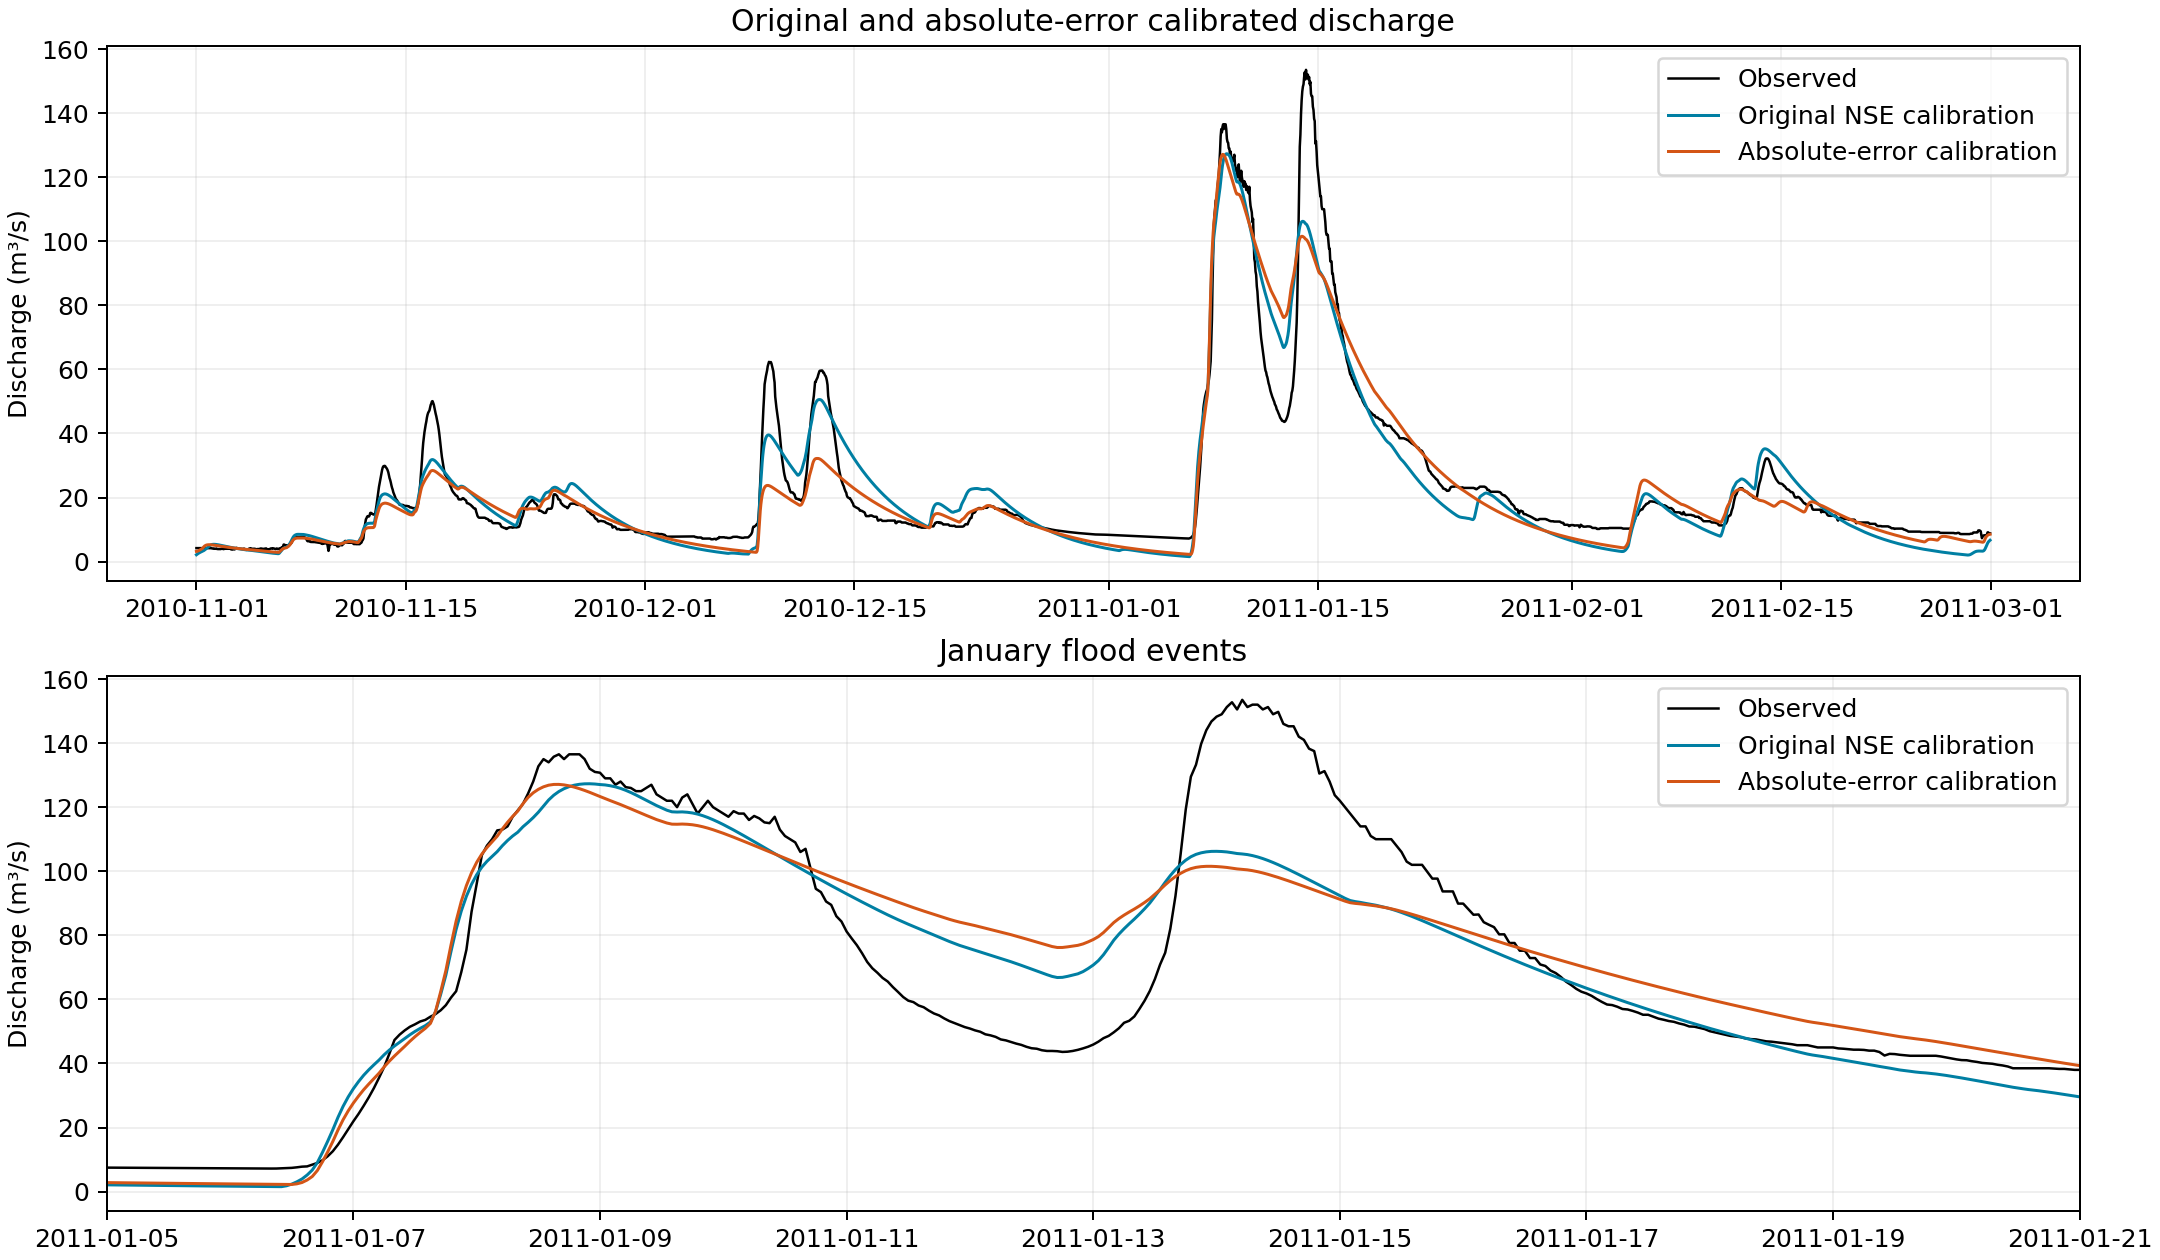
\includegraphics[width=\textwidth]{figures/absolute_de_fit.png}\caption{Original NSE calibration and absolute-error calibration.}\end{figure}
\clearpage
\subsection{Sensitivity before and after the adjustment}
The original columns use the original vector and $J=1-\mathrm{NSE}$; the absolute-error columns use the recalibrated vector and $J_{\mathrm{abs}}$. Each reports the mean and maximum absolute relative changes over 20 non-baseline perturbations around its respective vector.
\begin{center}\small\begin{tabular}{lrrrr}\toprule
Parameter & Original mean & Original max & Absolute mean & Absolute max\\\midrule
\param{sl0_fcy} & 5.81\% & 16.47\% & 2.18\% & 10.75\%\\
\param{snw_pmf} & 4.77\% & 14.64\% & 1.04\% & 2.80\%\\
\param{lrr_dre} & 4.22\% & 19.42\% & 3.05\% & 10.61\%\\\bottomrule\end{tabular}\end{center}
The mean and maximum relative changes decrease for all three parameters. The maximum for \param{snw_pmf} falls below 10\%; the other two remain slightly above. Objectives, baselines, and possibly feasible perturbation ranges differ, so these are not changes in standard NSE. A complete new ranking of all 18 parameters has not been computed.


\section{Open question}
Different random seeds can produce similar NSE values but substantially different parameter vectors. This experiment uses one saved vector. A different baseline requires new boundary checks and an assessment of whether the conclusions remain stable.
The data and scripts are in the accompanying Assignment 2 English folder. Result tables cover individual perturbations, sensitivity ranking, and combined perturbations.
\end{document}
